\begin{figure}[H]
    \centering
    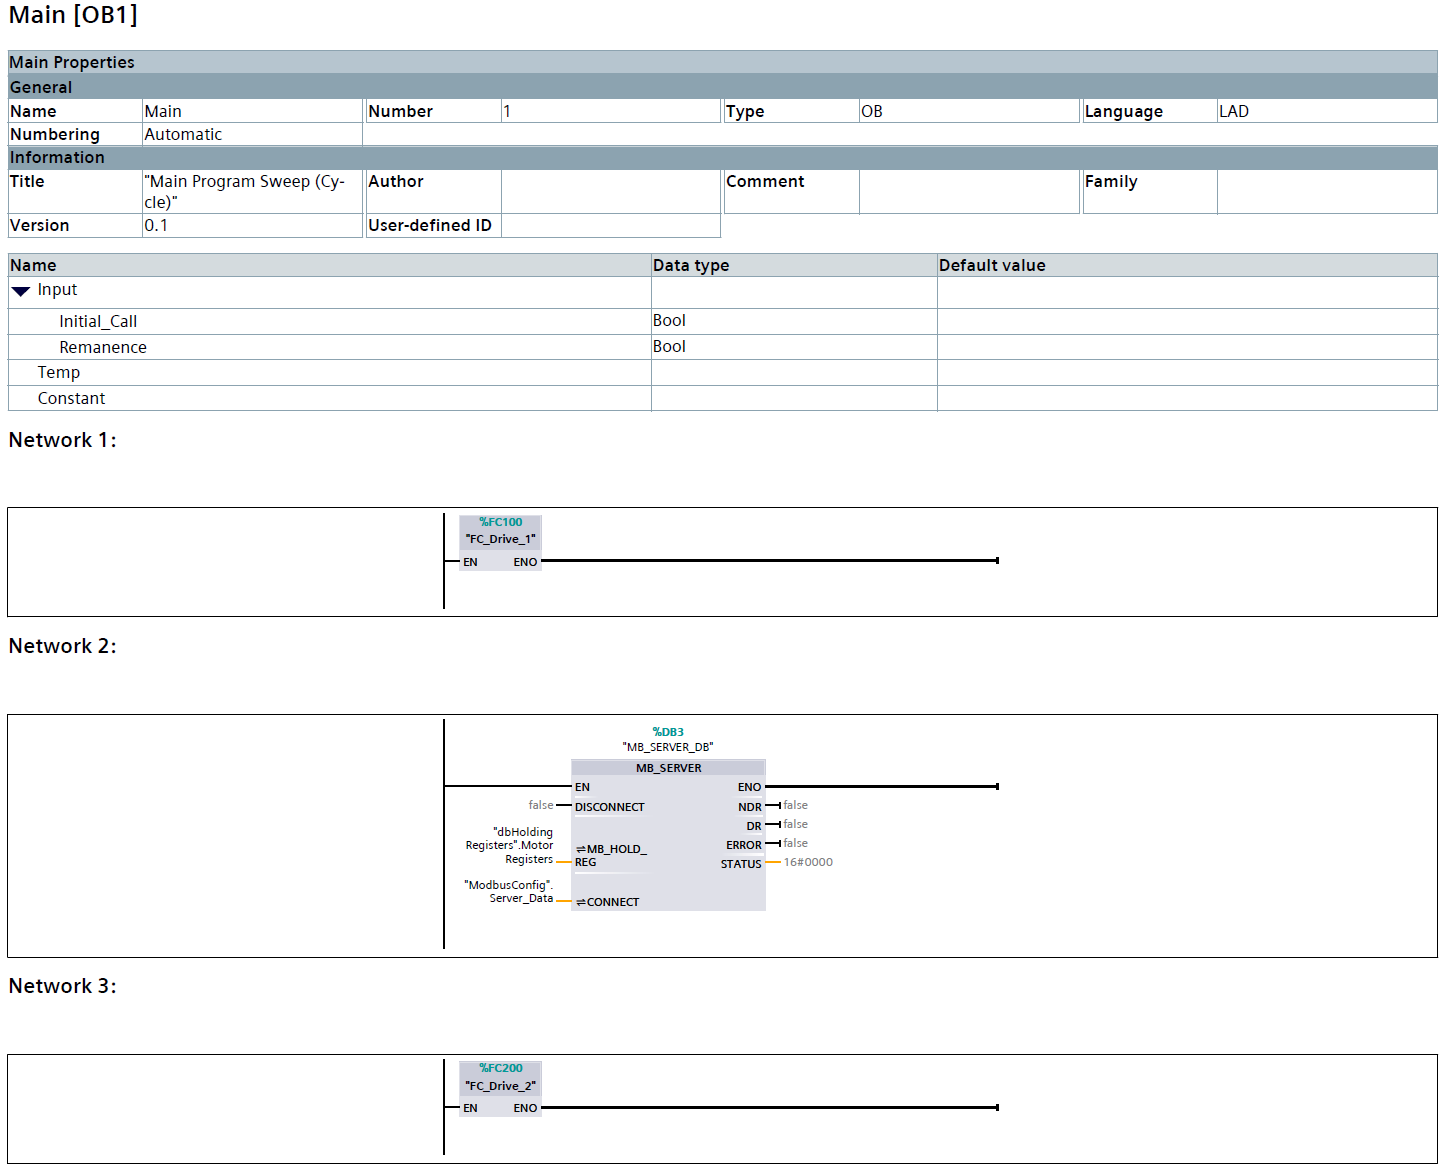
\includegraphics[width=0.5\linewidth]{FBDs/MainProgramSweep.PNG}
    \caption{''Main Program Sweep cycle'' på \acrshort{pls}-en.}
    \label{fig:OB1}
\end{figure}


\newgeometry{scale=0.75}
\thispagestyle{empty}
{%
\begin{figure}[H]
    \centering
    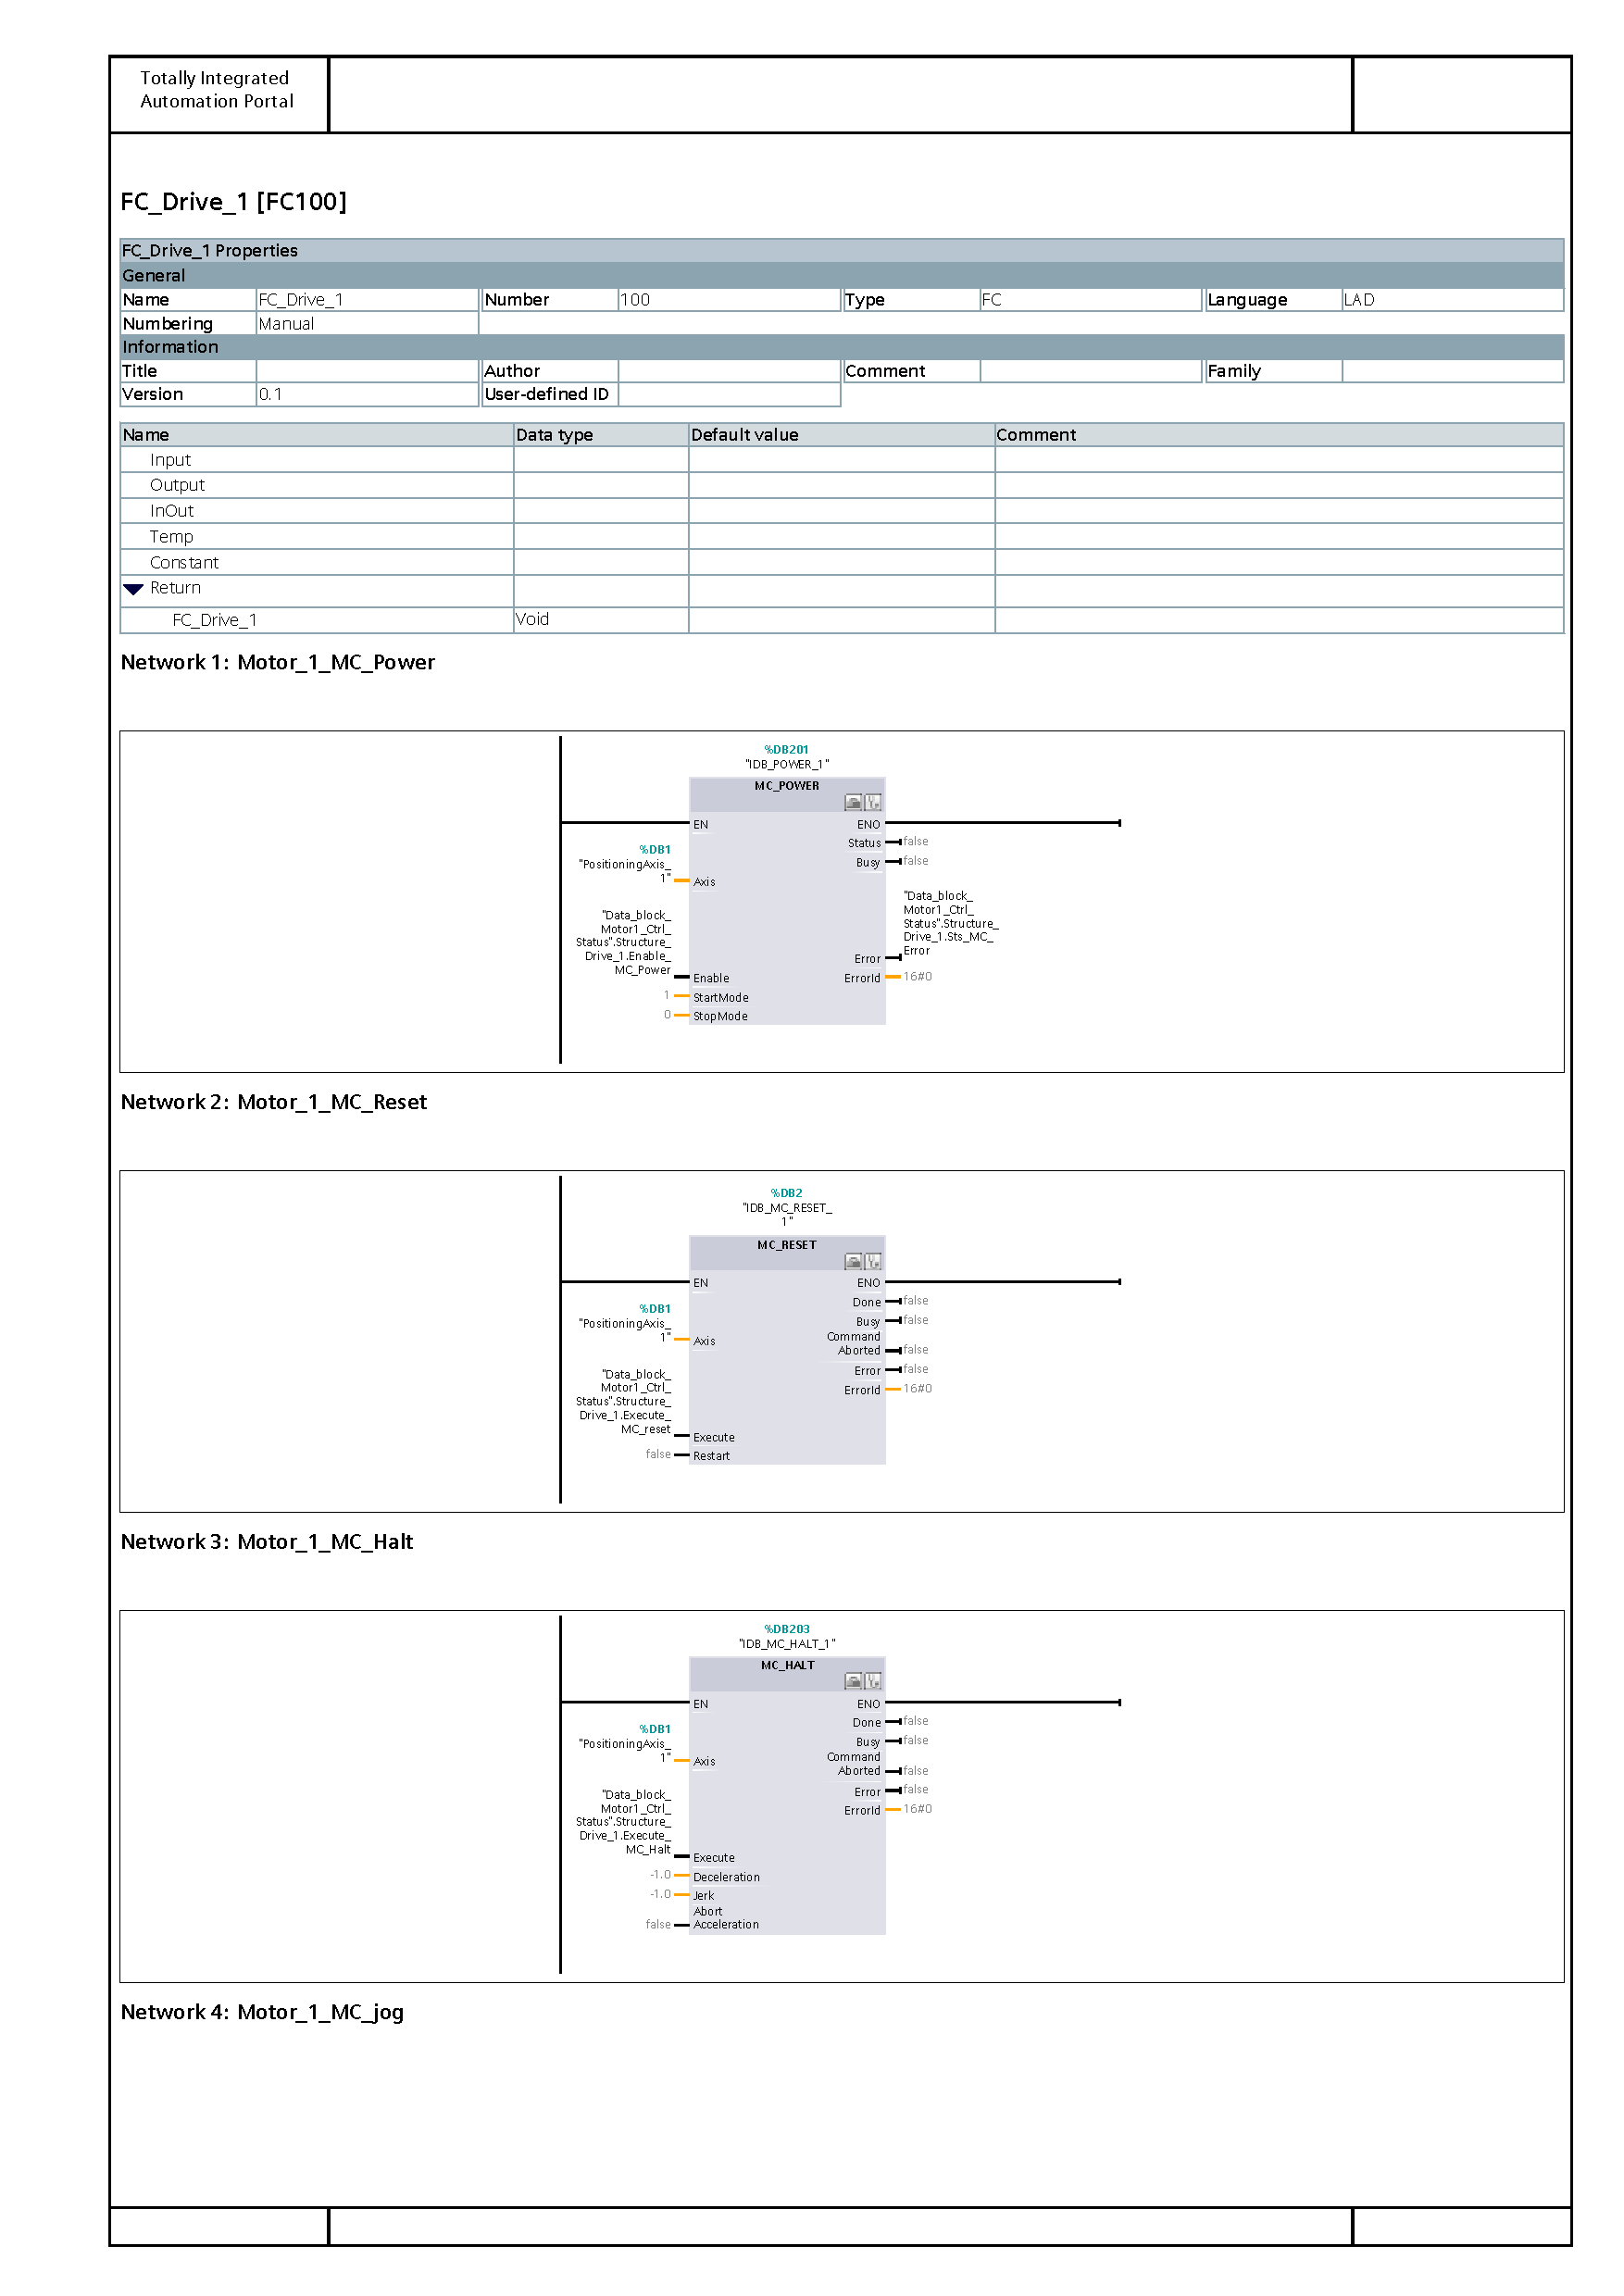
\includegraphics[page=1,scale=.5]{FBDs/FC_1.pdf}
    \caption{Funksjonsblokken som styrer Drive 1,  funksjonsblokk for Drive 2 lik med passende endring av variabler.}
    \label{fig:FC1}
\end{figure}
  \par
}
\includepdf[pages={2-4},scale=.75]{FBDs/FC_1.pdf}
\restoregeometry

\begin{figure}[H]
    \centering
    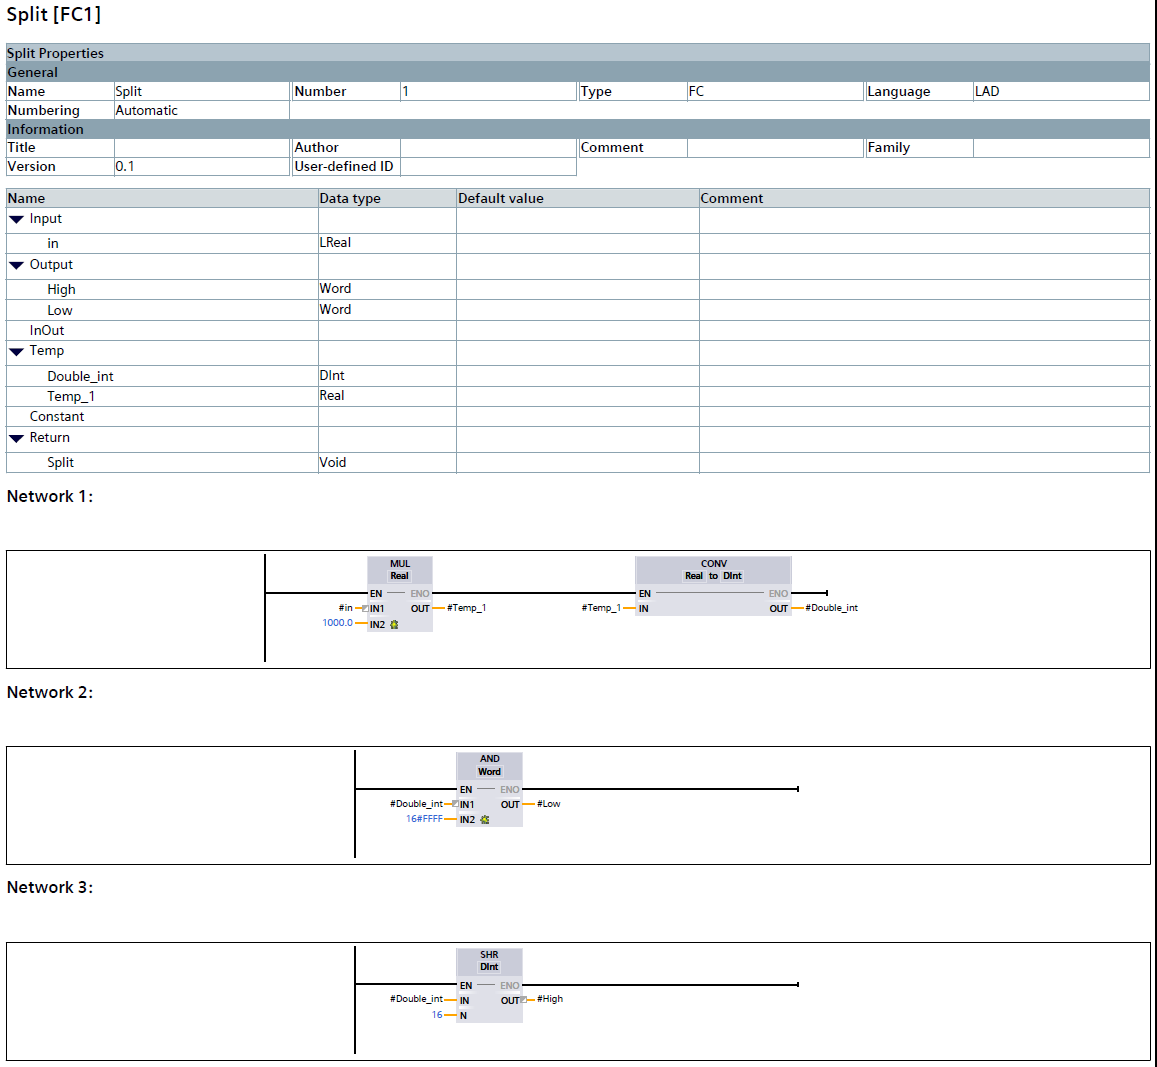
\includegraphics[width=0.5\linewidth]{FBDs/split.PNG}
    \caption{Funksjonsblokk for splitting av en 64-bit \Gls{lreal} til to 16-bit \gls{word}}
    \label{fig:split}
\end{figure}
\begin{figure}[H]
    \centering
    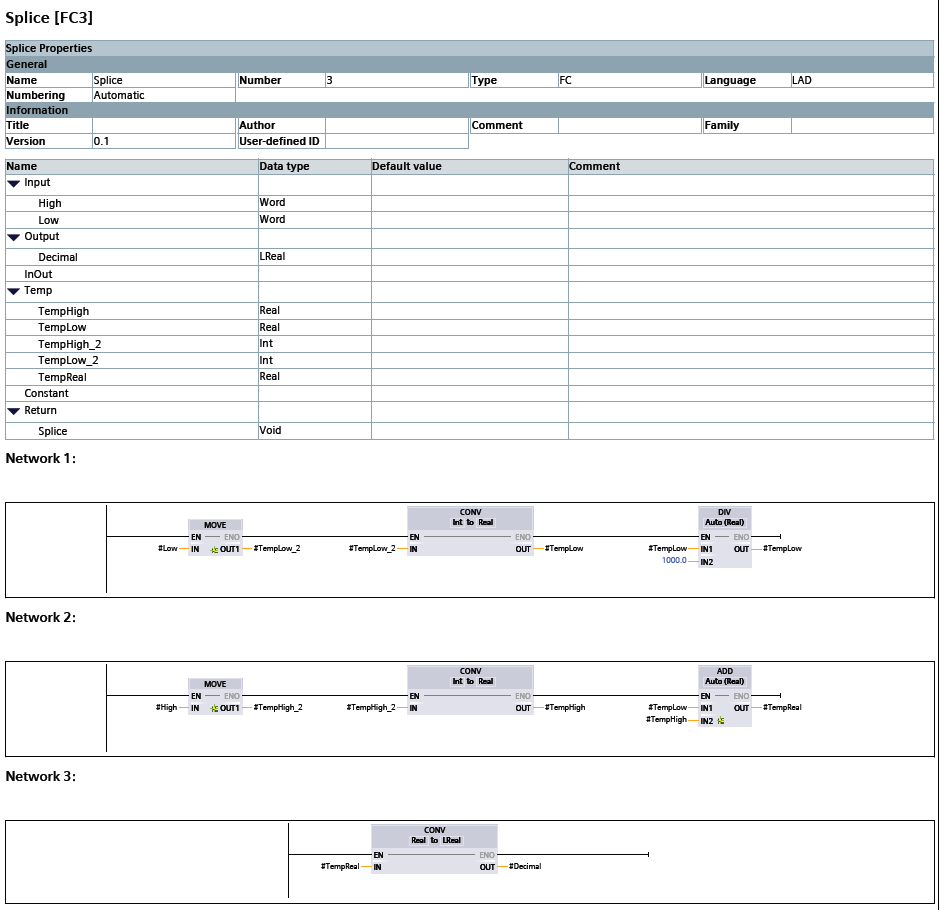
\includegraphics[width=0.5\linewidth]{FBDs/Splice.PNG}
    \caption{Funksjonsblokk for å spleise sammen en 32-bit \Gls{real}(flyttall) fra to 16 bit \glspl{word} før denne konverteres til en 64 bit \Gls{lreal}.}
    \label{fig:Splice}
\end{figure}

\begin{figure}[H]
    \centering
    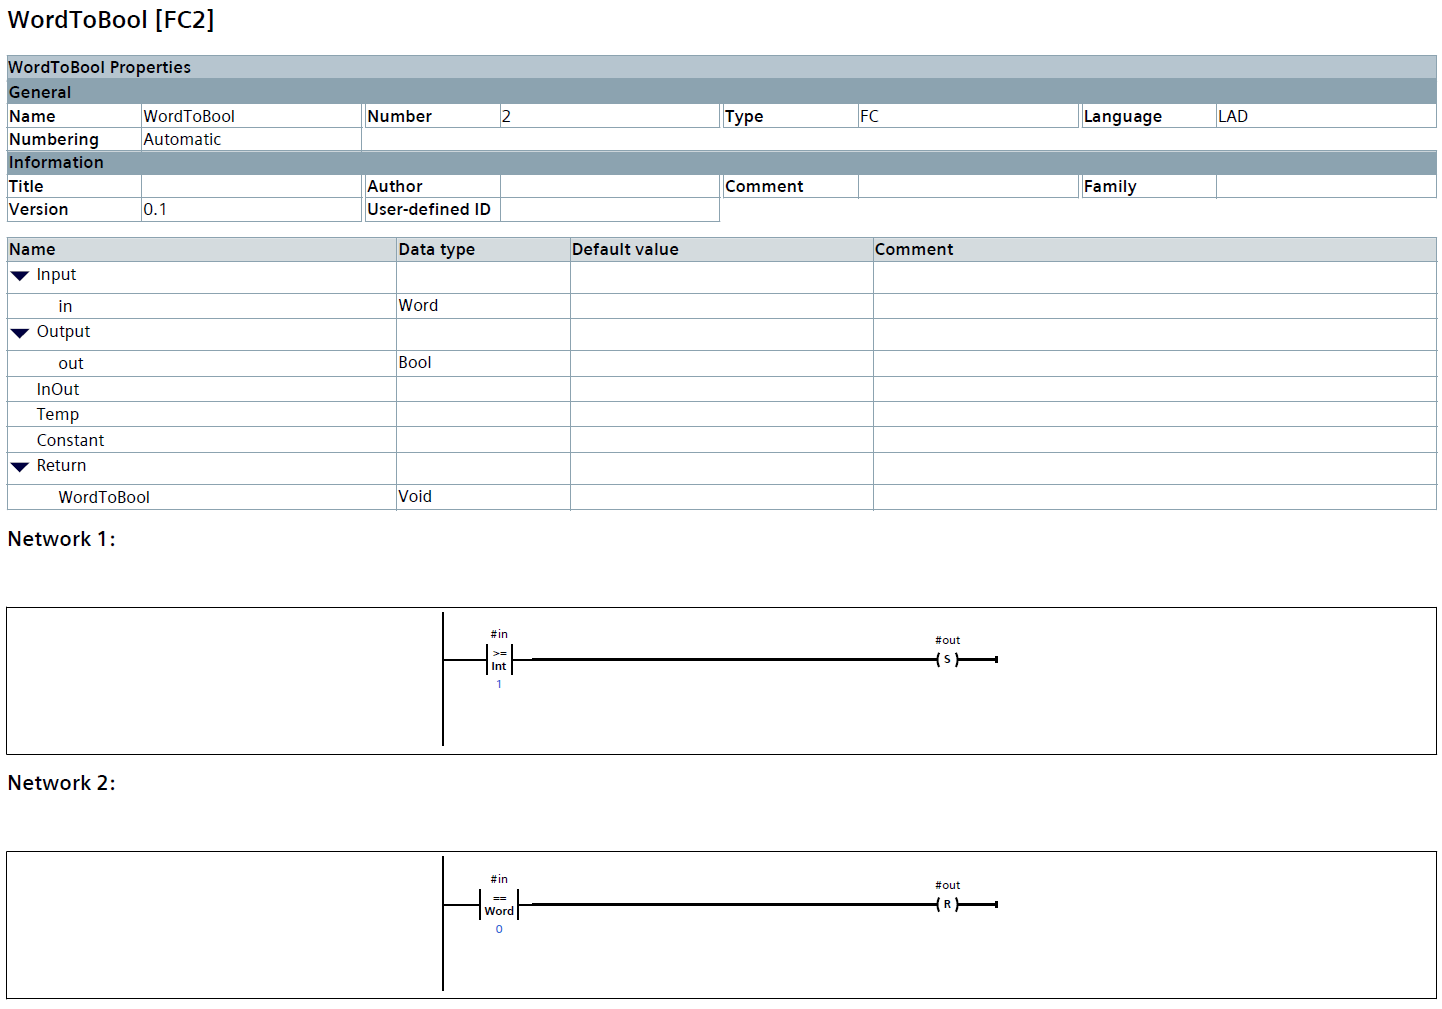
\includegraphics[width=0.5\linewidth]{FBDs/WordToBool.PNG}
    \caption{Funksjonsblokk for å konvertere et 16-bit \gls{word}(som kun tar veriene $0$  eller  $1$) til en 1-bit \glssk{bool} verdi}
    \label{fig:WTB}
\end{figure}